\pdfminorversion=5
\pdfinfoomitdate=1
\pdftrailerid{}
\documentclass[conference]{IEEEtran}
\IEEEoverridecommandlockouts

\usepackage{amsmath}
\usepackage{booktabs}
\usepackage{graphicx}
\usepackage{url}

\graphicspath{{figs/}}

\begin{document}

\title{Decoupling the Prediction Objective for\\
Inductive Temporal Link Prediction}

\author{%
\IEEEauthorblockN{Duong Viet Hoang\textsuperscript{*}}
\IEEEauthorblockA{Department of Computer Science\\
Da-Yeh University, Taiwan\\
Hoangduong4316@icloud.com\\
\textsuperscript{*}Corresponding author}
\and
\IEEEauthorblockN{Duong Viet Huy}
\IEEEauthorblockA{Department of Computer Science\\
Kent State University, United States\\
huydv6210@gmail.com}
\and
\IEEEauthorblockN{Lun-Min Shih}
\IEEEauthorblockA{Department of Computer Science\\
Da-Yeh University, Taiwan\\
Lmshih@mail.dyu.edu.tw}
}

\maketitle

\begin{abstract}
This paper examines a narrow design choice in temporal link prediction:
whether the prediction loss should update the temporal backbone. We compare a
coupled arm with a gradient-decoupled arm while holding the registered data,
split policy, negative sampling, training schedule, and evaluation endpoint
fixed. Across CoEdit, MOOC, and Wikipedia, the decoupled arm has the higher
mean inductive average precision in the selected runs. The result is a
within-protocol observation. It neither establishes causality nor supports a
claim against external implementations.
\end{abstract}

\begin{IEEEkeywords}
temporal graphs, link prediction, inductive evaluation, gradient decoupling,
research reproducibility
\end{IEEEkeywords}

\section{Introduction}

Temporal link predictors learn from ordered interactions and score candidate
edges at a later time. In an inductive split, at least one endpoint of a test
edge was absent from training. The setting therefore rewards representations
that transfer beyond the identities observed during optimization.

Most implementations let the link-prediction objective update every trainable
component. That choice is convenient, but it is not neutral: the prediction
head can shape the representation around shortcuts that are useful only for
the training population. We study a direct alternative. The decoupled arm
stops the score gradient at the backbone boundary, whereas the coupled arm
allows it to pass. The comparison changes that route and leaves the registered
evaluation protocol unchanged.

The contribution is deliberately bounded. We report the observed ordering of
the two registered arms on the current corpora and preserve the complete chain
from each table entry to a frozen aggregate, execution job, and checksum. We do
not use local proxy baselines to make external performance claims.

\begin{figure}[t]
  \centering
  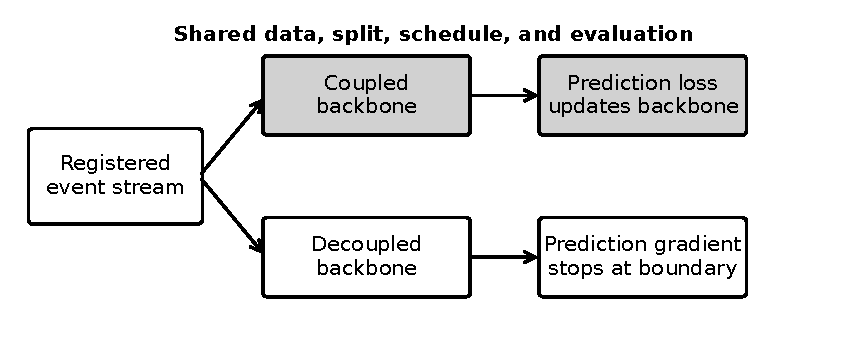
\includegraphics[width=\columnwidth]{protocol-contrast.pdf}
  \caption{The registered comparison changes the prediction-gradient route.
  Data handling and evaluation remain shared.}
  \label{fig:protocol}
\end{figure}

\section{Related Work}

Memory-based temporal models such as JODIE, DyRep, and TGN maintain evolving
node state, while attention and mixing architectures such as TGAT and
GraphMixer construct representations from temporal neighborhoods
\cite{kumar_jodie,trivedi_dyrep,rossi_tgn,xu_tgat,cong_graphmixer}. These
families motivate careful evaluation under inductive splits because node
identity and interaction history are not equally available at test time.

Stop-gradient operators and frozen representations have been studied as
optimization and transfer devices in other learning settings
\cite{chen_simsiam,alain_probes}. Here they serve a more limited purpose: they
define a controlled arm in a registered temporal-link experiment. The present
evidence does not establish that the result transfers to other architectures
or protocols.

\section{Registered Comparison}

Both arms use the same temporal backbone, corpus identities, chronological
split, negative-sampling policy, optimizer configuration, and metric
implementation. In the coupled arm, the link loss updates the backbone. In the
decoupled arm, the score path receives a detached backbone representation.
Figure~\ref{fig:protocol} shows this single experimental contrast.

The primary endpoint is inductive average precision. Each aggregate is formed
from the selected seed set, and dispersion is the sample standard deviation.
Runs outside the reconciled task matrix, including failed or superseded
attempts, cannot enter the aggregate silently.

\section{Results}

\begin{table}[t]
\centering
\caption{Inductive average precision in the registered comparison. Values are
mean $\pm$ sample standard deviation over the selected seeds.}
\label{tab:results}
\setlength{\tabcolsep}{4pt}
\begin{tabular}{llcc}
\toprule
Corpus & Training arm & Mean & SD \\
\midrule
CoEdit & Coupled & 0.9787 & 0.0021 \\
CoEdit & Decoupled & 0.9891 & 0.0016 \\
MOOC & Coupled & 0.9910 & 0.0047 \\
MOOC & Decoupled & 0.9947 & 0.0007 \\
Wikipedia & Coupled & 0.9967 & 0.0003 \\
Wikipedia & Decoupled & 0.9983 & 0.0003 \\
\bottomrule
\end{tabular}
\end{table}

The decoupled mean is higher for every corpus in
Table~\ref{tab:results}. The separation is largest on CoEdit and smaller on the
two standard interaction graphs. Figure~\ref{fig:ordering} presents the same
ordering without introducing additional reported values.

\begin{figure}[t]
  \centering
  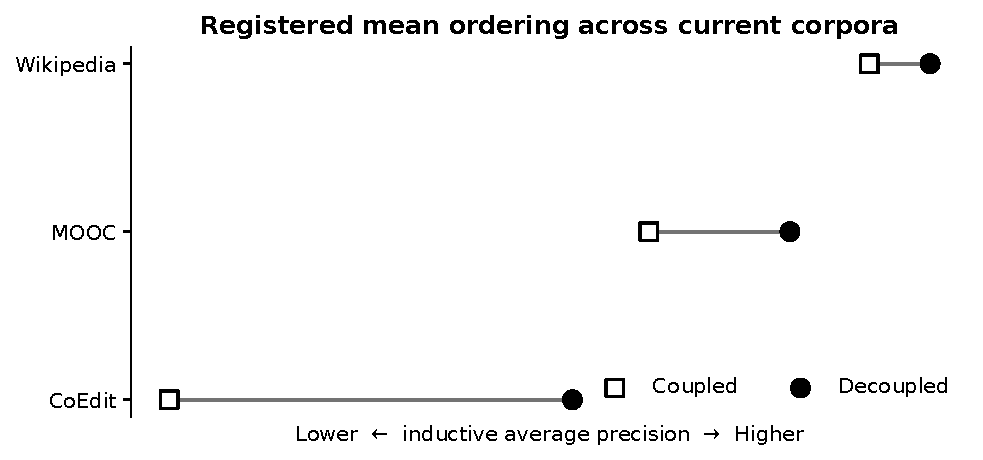
\includegraphics[width=\columnwidth]{inductive-ordering.pdf}
  \caption{Ordering of the registered inductive-AP means. Axis ticks and value
  labels are omitted because the audited values are reported in
  Table~\ref{tab:results}.}
  \label{fig:ordering}
\end{figure}

These observations do not identify a universal mechanism. In particular, the
current release does not support claims of irreversibility, superiority to
external baselines, hard-negative robustness, or state-of-the-art performance.
Those questions require their own registered implementations and evidence.

\section{Evidence Boundary}

The paper is built from an immutable evidence release. Each numeric occurrence
in Table~\ref{tab:results} resolves through an explicit selector to the frozen
aggregate produced by the registered scheduler reconciliation job. The release
also retains the protocol, resolved configuration, dependency lock, dataset
identities, environment record, attempt ledger, and final scheduler
accounting. The snapshot builder rejects a missing selector, a stale source
line, a checksum mismatch, or a value that does not reproduce the printed
rounding.

Dataset bytes are not distributed with the source repository. Acquisition is
fetch-only and requires the registered upstream digest. This boundary keeps
software licensing separate from dataset rights.

\section{Limitations}

The comparison covers one implementation, one protocol, and the current
registered corpora. It does not isolate which property of a corpus determines
the observed gap. It also does not compare against verified upstream baseline
implementations. The result should therefore be read as a controlled
within-system measurement rather than a general ranking of temporal graph
models.

\section{Conclusion}

Under the registered inductive protocol, the gradient-decoupled arm has a
higher mean average precision than the coupled arm on each current corpus.
The evidence supports that descriptive statement and no broader one. The
release and conference snapshot preserve the source, execution identity, and
numeric provenance needed to inspect the comparison independently.

\begin{thebibliography}{9}

\bibitem{kumar_jodie}
S. Kumar, X. Zhang, and J. Leskovec, ``Predicting dynamic embedding trajectory
in temporal interaction networks,'' in \emph{Proc. KDD}, 2019.

\bibitem{trivedi_dyrep}
R. Trivedi, M. Farajtabar, P. Biswal, and H. Zha, ``DyRep: Learning
representations over dynamic graphs,'' in \emph{Proc. ICLR}, 2019.

\bibitem{rossi_tgn}
E. Rossi, B. Chamberlain, F. Frasca, D. Eynard, F. Monti, and M. Bronstein,
``Temporal graph networks for deep learning,'' 2020.

\bibitem{xu_tgat}
D. Xu, C. Ruan, E. K\={o}rpeo\u{g}lu, S. Kumar, and K. Achan, ``Inductive
representation learning on temporal graphs,'' in \emph{Proc. ICLR}, 2020.

\bibitem{cong_graphmixer}
W. Cong, S. Zhang, J. Kang, B. Yuan, H. Wu, X. Zhou, H. Tong, and M. Mahdavi,
``Do we really need complicated model architectures for temporal networks?''
in \emph{Proc. ICLR}, 2023.

\bibitem{chen_simsiam}
X. Chen and K. He, ``Exploring simple Siamese representation learning,'' in
\emph{Proc. CVPR}, 2021.

\bibitem{alain_probes}
G. Alain and Y. Bengio, ``Understanding intermediate layers using linear
classifier probes,'' 2017.

\end{thebibliography}

\end{document}
